\documentclass[11pt]{article}

% Change "review" to "final" to generate the final (sometimes called camera-ready) version.
% Change to "preprint" to generate a non-anonymous version with page numbers.
\usepackage[review]{acl}

% Standard package includes
\usepackage{times}
\usepackage{latexsym}

% For proper rendering and hyphenation of words containing Latin characters (including in bib files)
\usepackage[T1]{fontenc}
% For Vietnamese characters
% \usepackage[T5]{fontenc}
% See https://www.latex-project.org/help/documentation/encguide.pdf for other character sets

% This assumes your files are encoded as UTF8
\usepackage[utf8]{inputenc}

% This is not strictly necessary, and may be commented out,
% but it will improve the layout of the manuscript,
% and will typically save some space.
\usepackage{microtype}

% This is also not strictly necessary, and may be commented out.
% However, it will improve the aesthetics of text in
% the typewriter font.
\usepackage{inconsolata}

%Including images in your LaTeX document requires adding
%additional package(s)
\usepackage{graphicx}
\usepackage{booktabs}
\usepackage{amsmath}
\usepackage{tikz}
\usetikzlibrary{arrows.meta,positioning,decorations.pathreplacing,calc}
\usepackage{enumitem}
% generated by tools/paper_numbers.py; do not edit
\newcommand{\dscrFiftyCR}{4}
\newcommand{\dscrFiftyPD}{37}
\newcommand{\dscrFiftyPR}{4}
\newcommand{\dscrFiftySD}{9}
\newcommand{\dscrMajorityCount}{35}
\newcommand{\dscrMajorityPct}{67.3}
\newcommand{\dscrVthreeCR}{4}
\newcommand{\dscrVthreePD}{35}
\newcommand{\dscrVthreePR}{4}
\newcommand{\dscrVthreeSD}{9}
\newcommand{\nPatAll}{91}
\newcommand{\nPatEligible}{55}
\newcommand{\nPatFifty}{54}
\newcommand{\nPatVthree}{52}
\newcommand{\permDscrMean}{15.0}
\newcommand{\permDscrN}{36}
\newcommand{\permDscrObserved}{14}
\newcommand{\permDscrP}{0.73}
\newcommand{\permHi}{37}
\newcommand{\permLo}{27}
\newcommand{\permMean}{32.4}
\newcommand{\permN}{95}
\newcommand{\permObserved}{32}
\newcommand{\permP}{0.64}
\newcommand{\tcmAgree}{52}
\newcommand{\tcmClassUnique}{18}
\newcommand{\tcmFollowAbsentGemmaTwelve}{11}
\newcommand{\tcmFollowAbsentGemmaTwentySeven}{21}
\newcommand{\tcmFollowAbsentMedGemma}{9}
\newcommand{\tcmFollowAbsentScout}{15}
\newcommand{\tcmFollowCorrectGemmaTwelve}{26}
\newcommand{\tcmFollowCorrectGemmaTwentySeven}{27}
\newcommand{\tcmFollowCorrectMedGemma}{9}
\newcommand{\tcmFollowCorrectScout}{24}
\newcommand{\tcmFollowIncorrectGemmaTwelve}{14}
\newcommand{\tcmFollowIncorrectGemmaTwentySeven}{14}
\newcommand{\tcmFollowIncorrectMedGemma}{8}
\newcommand{\tcmFollowIncorrectScout}{17}
\newcommand{\tcmN}{52}
\newcommand{\tcmNonCont}{17}
\newcommand{\tcmNonN}{17}
\newcommand{\tcmPdEsc}{35}
\newcommand{\tcmPdN}{35}
\newcommand{\vfourBpN}{94}
\newcommand{\vfourBpRatio}{1.4}
\newcommand{\vfourBpRho}{0.57}
\newcommand{\vfourConcordant}{130}
\newcommand{\vfourConcordantPct}{49}
\newcommand{\vfourExpCRN}{15}
\newcommand{\vfourExpCRSame}{12}
\newcommand{\vfourExpPDN}{161}
\newcommand{\vfourExpPDSame}{110}
\newcommand{\vfourExpPRN}{16}
\newcommand{\vfourExpPRSame}{2}
\newcommand{\vfourExpSDN}{76}
\newcommand{\vfourExpSDSame}{6}
\newcommand{\vfourFollowups}{268}
\newcommand{\vfourMajorityAIA}{25.8}
\newcommand{\vfourMajorityDSCR}{56.5}
\newcommand{\vfourMajorityLIL}{31.4}
\newcommand{\vfourMajorityTCM}{43.5}
\newcommand{\vfourNAIA}{62}
\newcommand{\vfourNDSCR}{62}
\newcommand{\vfourNLIL}{51}
\newcommand{\vfourNPJRF}{61}
\newcommand{\vfourNTCM}{62}
\newcommand{\vfourPatients}{62}
\newcommand{\vfourPending}{1}
\newcommand{\vfourPjrfAucLR}{0.547}
\newcommand{\vfourPjrfBase}{55.7}
\newcommand{\vfourPjrfBrierBase}{0.255}
\newcommand{\vfourPjrfBrierLR}{0.264}
\newcommand{\vfourPjrfN}{61}
\newcommand{\vfourSelectedAgree}{27}
\newcommand{\vfourTcmConfirm}{19}
\newcommand{\vfourTcmContinue}{27}
\newcommand{\vfourTcmEscalate}{16}
\newcommand{\vfourTcmLookupConf}{74.2}
\newcommand{\vfourTcmLookupEsc}{69.4}
\newcommand{\vfourTcmPdItems}{35}
\newcommand{\vfourUndetermined}{37}
\newcommand{\vthreeDiffGemmaTwelve}{$-$2.7}
\newcommand{\vthreeDiffGemmaTwentySeven}{+3.1}
\newcommand{\vthreeDiffMedGemma}{$-$1.9}
\newcommand{\vthreeDiffScout}{$-$3.1}
\newcommand{\vthreeDscrAccGemmaTwelve}{55.8}
\newcommand{\vthreeDscrAccGemmaTwentySeven}{65.4}
\newcommand{\vthreeDscrAccMedGemma}{15.4}
\newcommand{\vthreeDscrAccScout}{57.7}
\newcommand{\vthreeDscrCtxHurtGemmaTwelve}{$-$15.4}
\newcommand{\vthreeDscrCtxHurtGemmaTwentySeven}{$-$17.3}
\newcommand{\vthreeDscrCtxHurtMedGemma}{$-$3.8}
\newcommand{\vthreeDscrCtxHurtPGemmaTwelve}{0.021}
\newcommand{\vthreeDscrCtxHurtPGemmaTwentySeven}{0.012}
\newcommand{\vthreeDscrCtxHurtPMedGemma}{0.625}
\newcommand{\vthreeDscrCtxHurtPScout}{0.039}
\newcommand{\vthreeDscrCtxHurtScout}{$-$13.5}
\newcommand{\vthreeDscrPGemmaTwelve}{0.97}
\newcommand{\vthreeDscrPGemmaTwentySeven}{0.68}
\newcommand{\vthreeDscrPMedGemma}{1.00}
\newcommand{\vthreeDscrPScout}{0.95}
\newcommand{\vthreeTcmDscrOnlyGemmaTwelve}{+15.4}
\newcommand{\vthreeTcmDscrOnlyGemmaTwentySeven}{+26.9}
\newcommand{\vthreeTcmDscrOnlyMedGemma}{+1.9}
\newcommand{\vthreeTcmDscrOnlyScout}{+26.9}
\newcommand{\vthreeTcmGapGemmaTwelve}{34.6}
\newcommand{\vthreeTcmGapGemmaTwentySeven}{38.5}
\newcommand{\vthreeTcmGapMedGemma}{17.3}
\newcommand{\vthreeTcmGapPGemmaTwelve}{0.000}
\newcommand{\vthreeTcmGapPGemmaTwentySeven}{0.000}
\newcommand{\vthreeTcmGapPMedGemma}{0.004}
\newcommand{\vthreeTcmGapPScout}{0.004}
\newcommand{\vthreeTcmGapScout}{17.3}
\newcommand{\vthreeTcmNoDscrGemmaTwelve}{+1.9}
\newcommand{\vthreeTcmNoDscrGemmaTwentySeven}{+5.8}
\newcommand{\vthreeTcmNoDscrMedGemma}{$-$3.8}
\newcommand{\vthreeTcmNoDscrScout}{+3.8}


% If the title and author information does not fit in the area allocated, uncomment the following
%
%\setlength\titlebox{<dim>}
%
% and set <dim> to something 5cm or larger.

% \title{Do Medical MLLMs Read the Scan? Shortcut Controls on Brain-MRI Question Answering}
\title{Right Answer, No Image: Shortcut Learning in Brain-MRI Question
Answering}

% Author information can be set in various styles:
% For several authors from the same institution:
% \author{Author 1 \and ... \and Author n \\
%         Address line \\ ... \\ Address line}
% if the names do not fit well on one line use
%         Author 1 \\ {\bf Author 2} \\ ... \\ {\bf Author n} \\
% For authors from different institutions:
% \author{Author 1 \\ Address line \\  ... \\ Address line
%         \And  ... \And
%         Author n \\ Address line \\ ... \\ Address line}
% To start a separate ``row'' of authors use \AND, as in
% \author{Author 1 \\ Address line \\  ... \\ Address line
%         \AND
%         Author 2 \\ Address line \\ ... \\ Address line \And
%         Author 3 \\ Address line \\ ... \\ Address line}

\author{First Author \\
  Affiliation / Address line 1 \\
  Affiliation / Address line 2 \\
  Affiliation / Address line 3 \\
  \texttt{email@domain} \\\And
  Song Wang \\
  Affiliation / Address line 1 \\
  Affiliation / Address line 2 \\
  Affiliation / Address line 3 \\
  \texttt{email@domain} \\}

\begin{document}
\maketitle
\begin{abstract}
Multimodal LLMs are scored on medical image questions by final-answer accuracy, which cannot show whether an answer came from the image, the question text, or a shortcut, and removing the image says nothing about image use when the question cannot be answered from it. We build five-phase question chains from the LUMIERE glioblastoma cohort and first audit an expert-labeled version: only \vfourConcordantPct{}\% of expert RANO ratings can be reproduced from the enhancing lesion on the displayed slices, so image-removal results on those items cannot separate shortcut use from unanswerable questions. We rebuild the chains so that each answer key is a stated function of what the model sees: which sequence is shown, where the lesion lies on the displayed slice, the enhancement-based response category, a one-year mortality forecast scored by the Brier score, and a management rule that depends on both the response category and the time since chemoradiotherapy. Controls are fixed before the runs: a positive control that only the image can answer, matched donor-image swaps in which the donor's answer is always available, fixed-context comparisons, and fact-flip tests of the management rule, applied to four open-weight models. \ifnum\vfourPending=1 The v4 runs have not finished at the time of this draft; results are marked pending. \fi Items and keys are not clinician-validated.
\end{abstract}

\section{Introduction}
\label{sec:introduction}

Medical multimodal LLMs are usually scored on the letter they pick, which cannot separate a model that read the image and reasoned validly from one that used cues in the question or options, or guessed. Such shortcuts are well documented outside medicine: hypotheses alone beat chance on natural language inference \citep{gururangan2018annotation}, models adopt syntactic heuristics that fail on adversarial sets \citep{mccoy2019right}, and stated chain-of-thought often does not reflect what produced the answer \citep{turpin2023language}. In chest-radiograph question answering, models often rely on linguistic patterns or attend to irrelevant image regions, and textual and visual perturbation protocols exist for detecting this \citep{nguyen2025localizing}. A control that removes or swaps the image is only informative when the question can be answered from the image: if the displayed slice does not contain the evidence for the key, performance will not change for a model that reads images perfectly.

We ask whether accuracy on brain-MRI questions reflects reading the scan or a shortcut, and we treat answerability as a property to be built and audited, not assumed. We use the five clinical phases of OmniBrainBench \citep{peng2026omnibrainbench}, anatomical and imaging assessment (AIA), lesion identification and localization (LIL), diagnostic synthesis and causal reasoning (DSCR), prognostic judgment and risk forecasting (PJRF), and therapeutic cycle management (TCM), arranged as a same-patient chain on the LUMIERE glioblastoma cohort \citep{suter2022lumiere}. Our first construction drafted items with an LLM from expert RANO ratings and cohort records. Auditing it shows that the keys are not functions of the model-visible inputs (Section~\ref{sec:audit}), so we rebuilt it (Section~\ref{sec:v4}) and fixed the controls before running them (Section~\ref{sec:controls}).

The paper makes three contributions:
\begin{itemize}[leftmargin=*, itemsep=2pt, topsep=2pt]
    \item An answerability audit of an expert-labeled brain-MRI chain: an enhancement-based rule applied to the displayed slices reproduces the expert RANO category for only \vfourConcordantPct{}\% of \vfourFollowups{} follow-ups, and the released benchmark's groupings cannot support same-patient chains at all (2 verifiable cross-phase links in 6,823 questions).
    \item A chain in which every key is a stated function of the model-visible inputs, and a control suite fixed in advance: a positive control that only the image can answer, matched donor-image swaps with the donor's answer always available, fixed-context comparisons, and fact-flip tests that separate use of the diagnosis label from use of other supplied facts.
    \item \ifnum\vfourPending=1 Results on four open-weight models (pending at the time of this draft). \else Results on four open-weight models (Section~\ref{sec:results}). \fi The KAB vocabulary, adaptation and gating metrics we proposed earlier are kept only as exploratory instruments (Appendix~\ref{sec:kab}).
\end{itemize}

\section{Related Work}
\label{sec:related-work}

\paragraph{Shortcuts and faithfulness.} A model can reach a label without doing the intended task: hypothesis-only baselines beat the majority class on many NLI datasets \citep{poliak2018hypothesis, gururangan2018annotation}, models trained on such data adopt heuristics that fail on HANS \citep{mccoy2019right}, and biasing features in the input change chain-of-thought answers without appearing in the explanation \citep{turpin2023language}.

\paragraph{Answering without the image.} In visual question answering, language priors let models answer without the image, and \citet{goyal2017making} rebalanced the data so each question has two images with different answers. \citet{chen2024right} find that visual content is unnecessary for many samples in popular multimodal benchmarks. In medicine, \citet{yan2025worse} show that state-of-the-art models score below random guessing on specialized diagnostic questions when ground-truth questions are paired with adversarial counterparts, \citet{jin2024hidden} find flawed rationales in 35.5\% of GPT-4V's correct answers, and \citet{nguyen2025localizing} introduce textual and visual perturbation tests for chest-radiograph questions. Their items are single questions; we apply the same logic to a same-patient chain and add a positive control, matched swaps, and interventions on the stated clinical facts.

\paragraph{Brain benchmarks and same-patient continuity.} OmniBrainBench \citep{peng2026omnibrainbench} is a brain-imaging benchmark organized around a five-phase clinical workflow (15 modalities; 6,823 closed-ended questions). Its supplement describes a patient-level extension on the ADNI Alzheimer's cohort; the authors' repository provides label-generation code but no question data, and we did not evaluate it. LUMIERE \citep{suter2022lumiere} and MU-Glioma-Post \citep{muglioma2025post} provide real longitudinal glioma data with treatment and outcomes but no question layer.

\section{Building Answerable Chains from LUMIERE}
\label{sec:lumiere}

\paragraph{Why not OmniBrainBench.} A chain needs one patient's phases. We checked whether any image is shared across questions of different phases within a grouped case: of 6,823 closed-ended questions only 2 verifiable cross-phase patient links exist (both in VQA\_RAD, one AIA and one LIL question each), and a second method based on filename identifiers agreed; the counts are lower bounds (Appendix~\ref{sec:app-compat}). Each sub-corpus was built for one task, so a patient is essentially asked one phase-type of question. This is an incompatibility between the released groupings and our evaluation, not a defect in a promise its authors made.

\paragraph{LUMIERE.} LUMIERE \citep{suter2022lumiere} has 91 glioblastoma patients with longitudinal MRI (T1, contrast-enhanced T1, T2, FLAIR), automated segmentations (DeepBraTumIA and HD-GLIO-AUTO; \citealp{suter2022lumiere, kickingereder2019automated}), RANO ratings by one neuroradiologist \citep{wen2010updated}, and overall survival for most patients. Segmentations are automated and were not manually verified; the ratings are expert-assigned.

\subsection{Audit: are the expert labels answerable from the displayed slices?}
\label{sec:audit}

Our first item set (\texttt{v3}, Appendix~\ref{sec:app-v3}) let an LLM draft each phase's question from the expert RANO rating, the volume change between two segmentations, and cohort records. Three properties make its keys unanswerable from what the model sees. (i)~LIL asked for whole-lesion volume change, which one 2D slice per timepoint does not determine. (ii)~AIA had one fixed answer for every patient. (iii)~DSCR used the expert rating, which need not follow from the enhancing lesion. We measured (iii): on the axial slice with the largest enhancing area at each scan, we computed the RANO bidimensional product (longest diameter times longest perpendicular diameter) of the largest enhancing component and applied the enhancement criteria (progression: at least 25\% above the smallest earlier measurement, the nadir, or a new measurable lesion; response against the post-operative baseline; measurable means at least 10 by 10 mm). Of \vfourFollowups{} first-line follow-ups (one per rated, imaged timepoint before any second surgery), \vfourUndetermined{} are undetermined because no measurable enhancing disease exists on the baseline or nadir scan, and the rule reproduces the expert category for \vfourConcordant{} (\vfourConcordantPct{}\%): progressive disease \vfourExpPDSame{} of \vfourExpPDN{}, complete response \vfourExpCRSame{} of \vfourExpCRN{}, stable disease \vfourExpSDSame{} of \vfourExpSDN{}, partial response \vfourExpPRSame{} of \vfourExpPRN{}. The remaining ratings rest on evidence outside contrast enhancement on the displayed slices, such as T2/FLAIR progression, the choice of reference scan, clinical status and steroid dose. LUMIERE documents that one neuroradiologist rated the studies but not what information they used, so we do not say which. Our automated product correlates only moderately with the diameters the rater recorded for the target lesion (Spearman \vfourBpRho{} over \vfourBpN{} follow-ups; ours is a median \vfourBpRatio{} times larger), which is a limit on the segmentation-based keys. Agreement is a proxy: it does not show that the rule is right where the two disagree.

\subsection{The \texttt{v4} item set}
\label{sec:v4}

Each key is a stated function of the inputs the model receives (Table~\ref{tab:phases}). All random choices use fixed seeds and never look at model output.

\begin{table*}[t]
\centering
\footnotesize
\setlength{\tabcolsep}{3pt}
\begin{tabular}{p{0.7cm}p{4.6cm}p{4.4cm}p{4.4cm}r}
\toprule
Phase & Question & Model-visible inputs & Key & $n$ \\
\midrule
AIA & Which MRI sequence is shown? & one axial slice (T1, T1 after contrast, T2 or FLAIR) & the sequence rendered (balanced) & \vfourNAIA{} \\
LIL & Hemisphere and anterior/posterior half of the main tumor region & follow-up contrast-enhanced T1 slice at the level of the largest tumor region & position of the largest tumor-core component on that slice, relative to the midline and the brain's front-to-back midpoint & \vfourNLIL{} \\
DSCR & RANO enhancement category at follow-up & baseline, nadir and follow-up slices at the level of the largest enhancing lesion; the RANO thresholds are stated & category from the bidimensional products on those slices & \vfourNDSCR{} \\
PJRF & Probability of death within 52 weeks of this scan & age, sex, MGMT, IDH, extent of resection, weeks since surgery; alive at the scan & recorded outcome; scored by Brier score, not accuracy & \vfourNPJRF{} \\
TCM & Next management step & the same clinical facts plus weeks since chemoradiotherapy; the category comes from the chain & rule: non-PD continue; PD within 12 weeks of radiotherapy repeat MRI first; PD later change therapy & \vfourNTCM{} \\
\bottomrule
\end{tabular}
\caption{The \texttt{v4} phases. Stems for AIA, LIL and DSCR contain no patient-specific fact and every option set contains every possible answer, so a swapped image never conflicts with the text and the donor's answer is always available.}
\label{tab:phases}
\end{table*}

\paragraph{Cohort.} Of the patients with a first-line follow-up (rated, imaged, before any second surgery, with an imaged post-operative reference scan), we select one follow-up per patient in strata defined by the TCM rule class (continue, repeat MRI first, change therapy) and by the DSCR category, with quotas fixed in advance and a fixed seed, giving \vfourPatients{} patients. Selection used tabular records and segmentation masks only. Progressive-disease follow-ups whose timing falls within 2 weeks of the 12-week window are left out.

\paragraph{Images.} Each image is an atlas-space axial slice, skull-stripped by the dataset authors with HD-BET \citep{isensee2019automated}, at 4$\times$ magnification with a 20\,mm scale bar, in radiological orientation (checked against the affine). Slice levels are those on which the key is computed.

\paragraph{AIA, LIL, DSCR.} AIA is the positive control: its key is the sequence rendered, uniform over four sequences, so text alone can reach only chance. LIL's key is the hemisphere and anterior/posterior half of the largest tumor-core component on the displayed slice; lesions within 10\,mm of a midline, smaller than 100\,mm$^2$ or crossing the midline are not asked about. DSCR's stem states the RANO enhancement criteria, and its key is the category computed from the bidimensional products. The expert rating is recorded for each item but is not the key.

\paragraph{PJRF.} The prediction time is the follow-up scan, the available information is what the stem states plus the model's earlier assessment, and the outcome is death within 52 weeks of the scan, from the LUMIERE survival record (which we assume shares its origin with the week numbering; censoring is not documented). The model picks one of four probability bins (midpoints .10, .30, .50, .80) and is scored with the Brier score, not by whether it picked a ``correct'' bin. The recorded outcome is death in \vfourPjrfBase{}\% of \vfourPjrfN{} patients; a leave-one-out logistic model on the stated facts reaches Brier \vfourPjrfBrierLR{} against \vfourPjrfBrierBase{} for the constant base rate (AUC \vfourPjrfAucLR{}), so these facts support little beyond the base rate at this sample size.

\paragraph{TCM.} LUMIERE records no treatment after chemoradiotherapy, so a documented treatment is not available and the key is a rule-based recommendation, not what was done: non-progressive disease continues adjuvant temozolomide; progressive disease within 12 weeks of completing radiotherapy is confirmed with repeat MRI before any change; later progressive disease prompts a change of therapy. The 12-week window is from the RANO criteria \citep{wen2010updated}, which also allow progression inside the window when new enhancement lies outside the radiation field; we cannot assess the field, so the rule is a simplification. Radiotherapy dates are not in LUMIERE, so the stem states the weeks since chemoradiotherapy under an assumed standard schedule (ending 10 weeks after surgery). The same diagnosis therefore maps to different actions depending on the stated timing (\vfourTcmConfirm{} repeat-MRI and \vfourTcmEscalate{} change-therapy items among \vfourTcmPdItems{} progressive-disease items), which lets a lookup of the category alone be told apart from use of the timing fact.

\section{Controls and Pre-specified Analysis}
\label{sec:controls}

The analysis plan (\texttt{paper/preregistration\_v4.md}) was written before any \texttt{v4} model run; its hash is recorded in the project log, and the file is not externally timestamped. Models are the four open-weight models of the earlier study (MedGemma-4B, Gemma-3-12B, Gemma-3-27B, Llama-4-Scout; 4-bit, greedy decoding, 800 tokens; unparseable responses score incorrect). Each condition asks one question with a manufactured upstream context, so a phase's effect is not mixed with the model's own earlier answers.

\begin{itemize}[leftmargin=*, itemsep=1pt, topsep=2pt]
    \item \textbf{E1, image effect} (AIA, LIL, DSCR): accuracy with the image minus text only, paired by patient, with a patient-bootstrap interval. The margin is $\pm10$ percentage points, fixed in advance; ``within margin'' requires the whole interval inside it, and the interval half-width is about $1.96\sqrt{d/n}$ for a share $d$ of items whose correctness differs, so at $n=62$ the margin is reachable only if $d\le14\%$. Holm correction over the 12 model-phase tests; other contrasts are descriptive and unadjusted, with exact McNemar tests \citep{mcnemar1947note} and Wilson intervals \citep{wilson1927probable} where a proportion is reported. \textbf{AIA is the positive control:} for a model whose AIA interval is not above zero, the test has not been shown to detect image use, and E1 on LIL and DSCR supports no conclusion about it.
    \item \textbf{E2, donor tracking}: swap the image for a donor's with a different key (one donor per patient and phase, same number of images); $G=1[\text{swap}=\text{donor key}]-1[\text{text only}=\text{donor key}]$, so the no-image prior is subtracted.
    \item \textbf{E3, use of stated facts} (TCM): with the true context, move the stated timing across the 12-week window (\emph{flip\_window}) or replace the stated category by one that maps to another action class (\emph{flip\_label}), and report the share of answers that move to the rule's new answer. A category lookup alone cannot: it reaches at most \vfourTcmLookupConf{}\% (\vfourTcmLookupEsc{}\% if it always escalates), the rule 100\%.
    \item \textbf{E4, upstream context}: true, randomly wrong (each earlier answer replaced by a seeded random incorrect option) or absent context.
    \item \textbf{E5, PJRF}: Brier score and skill against the leave-one-out base rate, and AUC.
\end{itemize}

The ordinary five-phase chain (own answers as context) is run with and without images as a secondary analysis; each arm regenerates its upstream answers, so later-phase differences are total effects through the chain.

\section{Results}
\label{sec:results}

\subsection{Reference values without a model}

Table~\ref{tab:baselines} gives what constants and lookups reach. AIA is uniform over four answers, DSCR's most common category is progressive disease for \vfourMajorityDSCR{}\% of items, and a category-only TCM lookup reaches at most \vfourTcmLookupConf{}\%.

\begin{table}[t]
\centering
\footnotesize
\setlength{\tabcolsep}{3pt}
\begin{tabular}{lrrl}
\toprule
Phase & $n$ & Chance & Most common key \\
\midrule
AIA & \vfourNAIA{} & 25.0 & \vfourMajorityAIA{}\% \\
LIL & \vfourNLIL{} & 25.0 & \vfourMajorityLIL{}\% \\
DSCR & \vfourNDSCR{} & 25.0 & \vfourMajorityDSCR{}\% \\
TCM & \vfourNTCM{} & 25.0 & \vfourMajorityTCM{}\% (lookup $\le$ \vfourTcmLookupConf{}\%) \\
PJRF & \vfourNPJRF{} & (Brier) & base rate \vfourPjrfBase{}\% \\
\bottomrule
\end{tabular}
\caption{Non-model references on the \texttt{v4} items: chance, share of the most common key, the ceiling of a category-only TCM lookup, and the PJRF base rate.}
\label{tab:baselines}
\end{table}

\subsection{Image controls and stated facts}

\ifnum\vfourPending=1
\fbox{\parbox{0.94\linewidth}{\small \textbf{Pending.} The \texttt{v4} model runs (E1 to E5) had not finished when this draft was generated. The tables below are filled by \texttt{tools/paper\_numbers.py} from \texttt{results/lumiere\_v4\_stats.json}; the conclusions in this subsection are to be written from them under the decision rules of Section~\ref{sec:controls}.}}
\fi

\begin{table*}[t]
\centering
\footnotesize
\setlength{\tabcolsep}{3pt}
\begin{tabular}{llrrrll}
\toprule
Model & Phase & $n$ & Image & Text-only & $\Delta$ [95\% CI] & Verdict \\
\midrule
MedGemma-4B & AIA / LIL / DSCR & -- & -- & -- & -- & -- \\
Gemma-3-12B & AIA / LIL / DSCR & -- & -- & -- & -- & -- \\
Gemma-3-27B & AIA / LIL / DSCR & -- & -- & -- & -- & -- \\
Llama-4-Scout & AIA / LIL / DSCR & -- & -- & -- & -- & -- \\
\bottomrule
\end{tabular}

\caption{E1: accuracy (\%) with the image and with text only, with no upstream context, and the paired difference in percentage points. AIA is the positive control.}
\label{tab:e1}
\end{table*}

\begin{table*}[t]
\centering
\footnotesize
\setlength{\tabcolsep}{3pt}
\begin{tabular}{llrrrrl}
\toprule
Model & Phase & $n$ & Own image & Swap: donor key & Text: donor key & Gain [95\% CI] \\
\midrule
MedGemma-4B & AIA / LIL / DSCR & -- & -- & -- & -- & -- \\
Gemma-3-12B & AIA / LIL / DSCR & -- & -- & -- & -- & -- \\
Gemma-3-27B & AIA / LIL / DSCR & -- & -- & -- & -- & -- \\
Llama-4-Scout & AIA / LIL / DSCR & -- & -- & -- & -- & -- \\
\bottomrule
\end{tabular}

\caption{E2: share of answers (\%) that equal the donor's key when the image is swapped, and when there is no image; the gain is the difference in percentage points.}
\label{tab:e2}
\end{table*}

\begin{table}[t]
\centering
\footnotesize
\setlength{\tabcolsep}{3pt}
\begin{tabular}{lccccc}
\toprule
 & \multicolumn{3}{c}{TCM acc.\ (\%)} & \multicolumn{2}{c}{Follows rule (\%)} \\
\cmidrule(lr){2-4}\cmidrule(lr){5-6}
 & true & wrong & none & label & timing (PD) \\
\midrule
MedGemma-4B & -- & -- & -- & -- & -- \\
Gemma-3-12B & -- & -- & -- & -- & -- \\
Gemma-3-27B & -- & -- & -- & -- & -- \\
Llama-4-Scout & -- & -- & -- & -- & -- \\
\bottomrule
\end{tabular}

\caption{E3: TCM accuracy under true, random wrong and absent upstream context, and the share of answers that move to the rule's answer after the stated category is changed (label) or the stated timing crosses the 12-week window (timing, progressive-disease items).}
\label{tab:e3}
\end{table}

\begin{table}[t]
\centering
\footnotesize
\setlength{\tabcolsep}{3pt}
\begin{tabular}{lccccc}
\toprule
Model & $n$ & Brier & Base rate & Skill & AUC \\
\midrule
MedGemma-4B & -- & -- & -- & -- & -- \\
Gemma-3-12B & -- & -- & -- & -- & -- \\
Gemma-3-27B & -- & -- & -- & -- & -- \\
Llama-4-Scout & -- & -- & -- & -- & -- \\
\bottomrule
\end{tabular}

\caption{E5: PJRF Brier score with the true upstream context, against the leave-one-out constant base rate; skill $=1-$ Brier / base-rate Brier.}
\label{tab:e5}
\end{table}

\subsection{What the first item set showed}
\label{sec:v3-summary}

On \texttt{v3} (Appendix~\ref{sec:app-v3}; exploratory, with a margin chosen after seeing the intervals) removing the images changed accuracy by \vthreeDiffScout{}, \vthreeDiffGemmaTwentySeven{}, \vthreeDiffGemmaTwelve{} and \vthreeDiffMedGemma{} percentage points for Llama-4-Scout, Gemma-3-27B, Gemma-3-12B and MedGemma-4B. Given the audit above this is what one would see whether or not the models read the images, and we draw no shortcut conclusion from it. Two \texttt{v3} results are about the items' structure. TCM keys follow the DSCR category by construction (\tcmAgree{} of \tcmN{} keys map from the category to their action class), and accordingly correct upstream context beats forced-wrong context for all four models. DSCR is a class-imbalanced phase: progressive disease is the key for \dscrMajorityCount{} of \nPatVthree{} items (\dscrMajorityPct{}\%), above every model's DSCR accuracy. The motivation for the \texttt{v4} controls is that neither result can tell use of the category from use of the other stated facts.

\section{Conclusion}
\label{sec:conclusion}

Accuracy on an expert-labeled brain-MRI chain cannot show whether models read the scan: only \vfourConcordantPct{}\% of expert RANO ratings are reproducible from the enhancing lesion on the displayed slices, and the benchmark we started from cannot support same-patient chains. We rebuilt the chain on LUMIERE so that every key is a stated function of the model-visible inputs, and fixed a control suite in advance, with a positive control that only the image can answer, matched donor swaps, fixed-context comparisons and fact-flip tests of a management rule. \ifnum\vfourPending=1 The results of the four-model runs are pending at the time of this draft. \fi Clinician review of the keys, and in particular of the management rule and the assumed radiotherapy schedule, is the outstanding step, and proprietary models are not run. The controls apply to any chain-structured medical benchmark whose keys are made answerable from its inputs.


\section*{Limitations}
\label{sec:limitations}

\textbf{Clinician review is outstanding.} No clinician has judged whether each question is answerable from the inputs shown or whether each key is right; ``answerable by construction'' means only that each key is a stated function of the inputs. The functions rest on automated segmentation (DeepBraTumIA), whose errors propagate to the LIL and DSCR keys. The enhancement rule ignores T2/FLAIR change, clinical status and steroid dose, abstains where no measurable enhancing disease exists, and reproduces the expert category for \vfourConcordantPct{}\% of follow-ups; agreement does not show that the rule is right where the two disagree, and the expert rating is recorded but is not the key.

\textbf{The management key is a rule, not a documented treatment.} LUMIERE records no treatment after chemoradiotherapy. The TCM key rests on an assumed radiotherapy schedule (ending 10 weeks after surgery) and on a simplified reading of the 12-week RANO window, which also allows progression inside the window when new enhancement lies outside the radiation field. The PJRF outcome assumes that survival time and scan weeks share the surgery-week origin, and censoring is not documented. With \vfourPjrfN{} patients the stated facts do not support a forecast better than the base rate (leave-one-out Brier \vfourPjrfBrierLR{} against \vfourPjrfBrierBase{}), so PJRF can only show that a model is not worse than a constant.

\textbf{Power and scope.} With 51 to 62 patients per phase, the pre-specified $\pm10$-point margin is reachable only when few items differ between arms, and several cells will be inconclusive. The positive control tests one skill, sequence identification; passing it does not show that a model can read lesions. The donor images come from different patients, so anatomy differs beyond the tested feature; stems in the text-only arm still refer to images. Patients are from one center and the cohort was stratified by design; results cover four open-weight models at 4-bit, and larger models may need multi-GPU serving. Proprietary models were not run. Intervals treat patients as exchangeable.

\textbf{The first item set is exploratory.} Its items and distractors were LLM-drafted and are unreviewed; its equivalence margin was set after seeing the intervals; the donor-permutation, gating-causality, ablation and options-only analyses were added after seeing earlier results; 48 gating contrasts are uncorrected; the wrong-context condition used one fixed incorrect option; and the own-DSCR split of TCM accuracy is confounded by patient difficulty. KAB's ontology coverage is a string-matching metric that measures term validity, not correctness, and answer recoverability detects only inconsistency between reasoning and answer.

\section*{Ethics Statement}

This work evaluates the diagnostic reasoning of general-purpose and medical-domain language models on real, de-identified patient imaging data; it does not deploy, recommend, or endorse any model for clinical use, and no results in this paper should be interpreted as a clinical validation of any evaluated system. LUMIERE is used under its published non-commercial research license, and all patient data is accessed in its already de-identified, publicly released form; no new identifiable patient information is collected.

% Bibliography entries for the entire Anthology, followed by custom entries
%\bibliography{custom,anthology-overleaf-1,anthology-overleaf-2}

% Custom bibliography entries only
\bibliography{custom}

\appendix

\section{The First Item Set (\texttt{v3}) and Its Controls}
\label{sec:app-v3}

This appendix records the LLM-drafted item set of the earlier study and the controls run on it. It is exploratory: its answer keys are not functions of the model-visible inputs (Section~\ref{sec:audit}), and several of its analyses were added after seeing earlier results.

\subsection{Construction}
\label{sec:app-v3-construction}

LUMIERE \citep{suter2022lumiere} has 91 glioblastoma patients, 638 study dates, automated multi-sequence segmentation, and expert RANO ratings with rationale. Figure~\ref{fig:lumiere-pipeline} (Appendix~\ref{sec:dev-history}) summarizes the pipeline.

\paragraph{Facts.} Per-patient facts are extracted with provenance from LUMIERE's shipped data: segmentation masks already registered to MNI152 space reduce lesion location to a voxel lookup, and volumes ship precomputed. DSCR uses the released expert RANO ratings directly; we did not re-derive or audit them. The RANO criteria \citep{wen2010updated} draw on more than an image pair (reference and nadir scans, T2/FLAIR, clinical status, corticosteroid dose); the dataset does not document which of these the rater used, and Section~\ref{sec:audit} shows that the displayed slices reproduce the rating for only \vfourConcordantPct{}\% of follow-ups, so a DSCR answer cannot be assumed derivable from the model-visible inputs. PJRF and TCM facts come from the survival and Stupp-protocol records.

\paragraph{Cohort and drafting.} Of 91 patients, 55 meet the eligibility criterion (at least 3 RANO response-rated follow-ups and at least one timepoint with complete multi-sequence imaging); one has no timepoint with both and is dropped, leaving 54 patients and 269 drafted items. Claude 4.5 Sonnet drafts one multiple-choice item per phase with distractors from the facts. AIA, LIL, and DSCR are nearly programmatically derivable; PJRF and TCM need distractors informed by the glioblastoma prognosis and treatment literature (for example pseudoprogression), which the drafting prompt encodes.

\paragraph{Item construction.} For each patient we sample one random eligible timepoint that has both an expert RANO rating and complete imaging (fixed seed); always taking the last rated timepoint would make nearly every DSCR answer progressive disease. The resulting DSCR labels over the \nPatFifty{}-patient cohort are \dscrFiftyPD{} progressive disease, \dscrFiftySD{} stable disease, \dscrFiftyPR{} partial response, and \dscrFiftyCR{} complete response; over the \nPatVthree{} patients of the final set they are \dscrVthreePD{}, \dscrVthreeSD{}, \dscrVthreePR{} and \dscrVthreeCR{} (the two excluded patients were progressive disease). The LIL volume change is measured from each patient's latest post-operative scan before the follow-up, so that it reflects treatment response rather than resection; two patients without a matching post-operative segmentation are excluded, leaving 52 patients. DSCR, PJRF, and TCM answer keys do not depend on the LIL baseline. Drafted items pass through an automatic stem-leakage auditor that flags any stem or option restating the phase's own answer or an upstream phase's answer (a percent volume change, region name, change-direction word, RANO label, or survival duration); violations are fed back into the drafting prompt for up to eight retries, and the DSCR stem is a fixed template of clinical facts followed, since a later fix, by the rater\textquoteright s recorded findings (abbreviations expanded, no RANO label), because without that line most DSCR items were unanswerable from the images. The resulting item set (\texttt{v3}) has zero violations in every phase, which shows compliance with that auditor, whose rules the drafting loop was optimized against, not the absence of leakage. The development history (two sampling bugs, the leakier initial set \texttt{v2}, and the rebaselining) is in Appendix~\ref{sec:dev-history}.

\paragraph{Image rendering.} Each timepoint is one 2D axial slice: the slice with the largest tumor-mask area from the atlas-registered contrast-enhanced T1, rotated to radiological orientation and clipped to the 1st--99th percentile before scaling to 8-bit grayscale. There is no multi-slice or 3D rendering, and for the leak-controlled set the prompt states the radiological display convention. This bears on answerability: LIL asks about whole-lesion volume change computed from a 3D segmentation, which two maximum-area slices do not determine, so low LIL accuracy cannot be attributed to failure to use available evidence. The \texttt{v4} set replaces these keys (Section~\ref{sec:v4}).

\subsection{Setup}
\label{sec:setup}

\paragraph{Models.} Four open-weight models served through Ollama at 4-bit (Q4\_K\_M): MedGemma-4B (the only medical fine-tune), Gemma-3-12B, Gemma-3-27B, and Llama-4-Scout (109B mixture-of-experts, 17B active); tags \texttt{medgemma:4b}, \texttt{gemma3:12b}, \texttt{gemma3:27b}, \texttt{llama4:scout}, each on one RTX PRO 6000. Proprietary models (GPT-5, Claude 4.5 Sonnet, Gemini 2.5 Pro) are planned but not yet run. All models use one OpenAI-compatible interface with greedy decoding (temperature $0$) and an $800$-token budget, and the response schema asks for \texttt{answer} before grounding and reasoning so a truncated response still has an answer.

\paragraph{Failed responses.} A call is retried up to 3 times with exponential backoff. If the JSON fails to parse (truncation, or unescaped newlines, recovered by a lenient parse), we salvage the answer letter by regex; if that fails the item is scored incorrect, not excluded, so a model prone to malformed output does not get an easier denominator. Salvaged answers are scored on the salvaged letter. (The evaluator's per-run report instead drops parse-error items from a phase's denominator, which lowers MedGemma-4B's image and text-only accuracy from 34.2\% and 36.2\% to 33.1\% and 35.8\% (3 and 1 items); we report the per-question basis.)

\paragraph{Knowledge bases.} RadLex (RSNA OWL, downloaded 2026-08-05) and the NCI Thesaurus \citep{sioutos2007nci} (OWL v26.07d) are used as-is; the aligner raises an error if either is missing.

\subsection{Controls}
\label{sec:grounding-test}

The vocabulary and consistency metrics test whether stated reasoning is internally consistent, not whether it derives from the image; recoverability in particular passes any response whose reasoning restates its chosen option. We therefore run controls on the leak-controlled item set, identically across the four models: a leakage audit, a text-only ablation, an evidence fact-check, counterfactual image substitution with a donor-permutation test, a repeated-run control, a gating-causality intervention with a TCM ablation, and an options-only baseline.

\paragraph{Stem-leakage audit.} The auditor of Appendix~\ref{sec:app-v3-construction} doubles as a diagnostic: an item whose stem or upstream context already states the answer tests nothing about image use. Running it on both item sets is a controlled manipulation for the other checks.

\paragraph{Text-only ablation.} We strip all images and compare accuracy with the image-present run on the same items. Both arms are non-gated so every phase is scored. Chain context is regenerated from each arm's own earlier answers, so later-phase differences combine a same-phase effect with propagated upstream effects. If the patient-clustered paired difference lies within an equivalence margin, the image is not necessary for the answer on this item set; a nonsignificant difference alone would not show this.

\paragraph{Evidence fact-check.} For each checkable claim in a response's \texttt{visual\_grounding} and \texttt{reasoning} (hemisphere or region statements, and measurements with units) we record two properties: \emph{availability} (already in the stem, options, or upstream context shown) and \emph{record status} (supported, contradicted, unmatched, or unverifiable against the structured facts). Responses with no checkable claim are reported separately. The audit is deterministic pattern matching and does not interpret paraphrase (Appendix~\ref{sec:app-audit}).

\paragraph{Counterfactual-image substitution.} We replace each patient's image with a different real patient's (the \emph{donor}'s), keeping every text field, including timepoint labels, unchanged. A deterministic seeded pairing gives the donor an opposite-sign lesion-volume change. LIL and DSCR are the primary phases; AIA's answer is a fixed string and serves as a reference; PJRF and TCM mix same-phase and propagated upstream effects. The options remain the original patient's, so the donor's fully correct answer is generally absent and the donor's clinical facts in the stem are not substituted; truth-tracking is testable only at label level (volume-change direction for LIL, RANO category for DSCR). The outcomes are the flip rate and, among flips, agreement with the donor's label, judged against a donor-permutation null: each patient's donor is redrawn uniformly from the patients with the opposite LIL direction, the observed flipped answers are held fixed, and agreement is recounted (20,000 replicates; one donor per patient shared across models and phases). A null in which a flip lands uniformly on another option would ignore that models skew toward common labels.

\paragraph{Repeated identical-input control.} For each model we re-run the own-image condition with identical inputs and greedy decoding (run tag \texttt{rep2}) to measure run-to-run variability.

\paragraph{Gating-causality experiment.}\label{sec:gating-causality} To test rather than impose the dependency between phases, we evaluate LIL, DSCR, PJRF, and TCM under three manufactured upstream-context conditions (the true upstream answers, a fixed incorrect option per upstream phase, no upstream context) with image, question, and options held fixed. If downstream accuracy does not differ across conditions, the assumed dependency is not supported. Contrasts are paired on the patient, with patient-clustered bootstrap intervals and exact McNemar tests, uncorrected for multiplicity.

\paragraph{TCM context ablation.} The TCM drafting prompt makes the correct treatment follow from the patient's disease course, so TCM may be answerable by looking up the upstream DSCR label. We rerun TCM with only the DSCR entry injected, or with every upstream entry except DSCR, under the true and incorrect conditions.

\paragraph{Options-only baseline.} The model sees only the four answer options, with no image, question stem, or chain context. Accuracy above chance or the majority rate would mean the options themselves leak the answer. We compare it with the same items shown with image and stem but no chain context (the ``absent'' condition above). Responses that cannot be parsed score incorrect, so a model with many parse failures gets a lower-bound score.

\paragraph{Analysis plan.} Before running the \texttt{v3} and counterfactual jobs we recorded a joint decision rule in our dated project log (\texttt{paper/update.md}, 2026-09-22): text-only accuracy within the confidence interval of image-present accuracy, evidence mostly restated from shown text, and a low, non-truth-tracking flip rate together indicate non-grounding; the opposite pattern indicates grounding. The log was not externally timestamped, so this is a prespecified analysis plan, not a preregistration. It used confidence-interval overlap; the $\pm8$pp margin below was adopted afterwards, after we had seen the intervals, and describes what the data can exclude rather than a prespecified test. The donor permutation, gating-causality, ablation, and options-only analyses were added after seeing earlier results and are exploratory.

\subsection{Results}
\label{sec:app-v3-results}

All results here use the leak-controlled (\texttt{v3}) item set and the four open-weight models. The initial item set (\texttt{v2}) failed the stem-leakage auditor at rates too high to treat its accuracy as informative about image use (Appendix~\ref{sec:dev-history}); \texttt{v3} clears every phase with zero violations, which shows compliance with that auditor, not that no leakage remains.

\begin{table}[t]
\centering
\footnotesize
\setlength{\tabcolsep}{3pt}
\begin{tabular}{lccc}
\toprule
Model & Image & Text-only & $\Delta$ [95\% CI] \\
\midrule
Llama-4-Scout & 48.8 & 51.9 & $-$3.1 [$-$7.3, +1.2] \\
Gemma-3-27B & 53.5 & 50.4 & +3.1 [$-$0.8, +7.3] \\
Gemma-3-12B & 48.1 & 50.8 & $-$2.7 [$-$7.3, +2.3] \\
MedGemma-4B & 34.2 & 36.2 & $-$1.9 [$-$5.8, +1.9] \\
\bottomrule
\end{tabular}

\caption{Non-gated accuracy (\%) with images versus text-only, and the paired difference $\Delta$ = image $-$ text-only in percentage points with its patient-clustered 95\% bootstrap interval (52 patients, 10,000 resamples). Accuracy is per question (Appendix~\ref{sec:setup}).}
\label{tab:textonly}
\end{table}

\begin{figure}[t]
\centering

\includegraphics[width=\linewidth]{figures/phase_effects.pdf}
\caption{Paired accuracy difference (image minus text-only, percentage points) by phase and model, with patient-clustered 95\% bootstrap intervals; right of zero means the image helped. Not adjusted for multiplicity across the 20 cells.}
\label{fig:phase-effects}
\end{figure}

\paragraph{Text-only ablation.} Table~\ref{tab:textonly} gives accuracy with and without images and Figure~\ref{fig:phase-effects} the paired per-phase differences; patients, not questions, are resampled because each contributes one question per phase. Three of four models score at least as high without the image (image minus text-only: Llama-4-Scout $-3.1$pp, Gemma-3-12B $-2.7$, MedGemma-4B $-1.9$). Gemma-3-27B is the exception ($+3.1$), concentrated in AIA ($+9.6$pp, $[-1.9,+21.2]$; 8 items right only with the image, 3 only without). Every overall interval includes zero; all fall within $\pm8$pp and none within $\pm5$pp. We chose the $\pm8$pp margin after seeing them, so it describes what the data exclude and is not a prespecified test, and 52 patients give limited power against a moderate effect. Across the 20 model-phase cells no interval lies entirely on the image-advantage side. A model gives the same answer with and without the image on 77--89\% of items and the same correct-or-incorrect outcome on 87--91\%; among items whose outcome differs, right-only-with-image and right-only-without-image are comparable (55 versus 67). Decoding is deterministic (repeated-run control below), so these changes come from removing the image; the image changes answers without changing net accuracy.

\paragraph{Repeated identical-input control.} All four models return identical answers on 260 of 260 questions (with identical correctness) when the own-image run is repeated, with 0 flips in every phase. Decoding is deterministic, so the noise floor for the answer-change comparisons in this section is zero; this does not bound sensitivity to small input perturbations.

\paragraph{Evidence fact-check.} 26--55\% of answers contain no checkable claim (MedGemma-4B 35\%, Gemma-3-12B 31\%, Gemma-3-27B 55\%, Llama-4-Scout 26\%); they are excluded from the claim-level denominators below. Among the remaining claims (251--668 per model), 75--87\% were available in shown text and match the record; 10--18\% were available in shown text yet contradict or fail to match the record (for example a wrong location repeated from an earlier turn, which a single ``copied'' label would hide); only 1--2\% were absent from shown text and match the record; and 2--6\% were absent and contradict or fail to match. The small share of novel, record-matching claims means the audit finds little evidence that stated evidence contains facts obtainable only from the image. It cannot show the converse: a model can inspect an image and choose wording that also appears in an option, and a novel claim that matches the record need not have been read from the image. The audit is descriptive, misses paraphrase, and is not validated against expert annotation.

\begin{table}[t]
\centering
\footnotesize
\setlength{\tabcolsep}{3pt}
\begin{tabular}{lccc}
\toprule
Model & AIA & LIL & DSCR \\
\midrule
MedGemma-4B & 17 [8, 29] & 12 [4, 21] & 6 [0, 13] \\
Gemma-3-12B & 10 [2, 17] & 37 [23, 50] & 27 [15, 38] \\
Gemma-3-27B & 17 [8, 29] & 42 [29, 56] & 25 [13, 37] \\
Llama-4-Scout & 10 [2, 17] & 23 [12, 35] & 12 [4, 21] \\
\bottomrule
\end{tabular}
\caption{Flip rate (\%) between own-image and donor-image runs with patient-clustered 95\% bootstrap intervals ($n=52$ per cell). AIA's answer does not depend on the image.}
\label{tab:flip}
\end{table}

\paragraph{Counterfactual-image substitution.} Table~\ref{tab:flip} gives flip rates. Because repeated identical runs agree exactly, every flip, including AIA's 10--17\%, is caused by the image change; AIA's answer is a fixed string, so its flips show that changing the image perturbs a response even when nothing answer-relevant differs. LIL (12--42\%) and DSCR (6--27\%) flip more often than AIA for Gemma-3-12B and Gemma-3-27B on both phases and for Llama-4-Scout on LIL, and no more often for MedGemma-4B; several intervals overlap AIA's. PJRF (4--23\%) and TCM (10--37\%) also flip, but their upstream context is regenerated under the swapped image.

Among the 95 flipped LIL and DSCR items, 32 (33.7\%) carry the donor's label, but the donor-permutation test gives a null mean of 32.4 (95\% range 27--37; one-sided $p=.64$): LIL 18 of 59 against 17.4 expected, DSCR 14 of 36 against 15.0. Which donor's image was shown does not matter beyond what the label base rates predict. (An earlier item-specific null, in which a flip lands uniformly on another option, put the expectation at 21.8\% and suggested a $+11.9$pp excess; it ignored that models skew toward common labels, such as progressive disease for \dscrMajorityPct{}\% of DSCR keys.) The LIL permutation is degenerate by the pairing rule, which fixes every donor's LIL direction opposite to the patient's, so only DSCR is informative about donor specificity. In LIL, 67.8\% of flips land on the original patient's own direction (47.2\% in DSCR, where the two patients' labels sometimes coincide), and 30.5\% of flips keep the same direction or RANO label and cannot track the swap. The check is limited by option availability (the donor's correct LIL option was among those shown for 0 of 52 patients, and its direction label for 37 of 52; for DSCR, 52 of 52 in both cases), by donor facts in the stem that were not substituted, and by 2 of 52 pairs in which one patient's LIL truth is a near-zero, ``stable'' change.

\begin{table}[t]
\centering
\footnotesize
\setlength{\tabcolsep}{2pt}
\begin{tabular}{lcccc}
\toprule
 & \multicolumn{3}{c}{TCM} & DSCR \\
\cmidrule(lr){2-4}\cmidrule(lr){5-5}
Model & c / w / a & $\Delta_{\text{DSCR}}$ & $\Delta_{\text{no DSCR}}$ & c / w / a \\
\midrule
MedGemma-4B & 33/15/25 & +1.9 & $-$3.8 & 15/21/19 \\
Gemma-3-12B & 62/27/19 & +15.4$^{*}$ & +1.9 & 50/65/65 \\
Gemma-3-27B & 63/25/33 & +26.9$^{*}$ & +5.8 & 54/63/71 \\
Llama-4-Scout & 60/42/33 & +26.9$^{*}$ & +3.8 & 50/62/63 \\
\bottomrule
\end{tabular}

\caption{Accuracy (\%) under correct (c), forced-wrong (w), and absent (a) upstream context ($n=52$). $\Delta$ is correct minus wrong TCM accuracy in points when only the DSCR entry ($\Delta_{\text{DSCR}}$) or every entry except DSCR ($\Delta_{\text{no DSCR}}$) is injected; $^{*}$ the patient-clustered 95\% interval excludes zero. Full-context TCM correct minus wrong is \vthreeTcmGapMedGemma{}, \vthreeTcmGapGemmaTwelve{}, \vthreeTcmGapGemmaTwentySeven{} and \vthreeTcmGapScout{} points (MedGemma-4B, Gemma-3-12B, Gemma-3-27B, Llama-4-Scout), all excluding zero. In the DSCR column the true context is the true answers of the earlier phases (AIA and LIL) supplied to DSCR, never DSCR\textquoteright s own label. Uncorrected.}
\label{tab:gating}
\end{table}

\paragraph{Gating-causality and TCM.} Table~\ref{tab:gating} gives the interventions. TCM accuracy depends on upstream context for all four models: correct context beats forced-wrong context by \vthreeTcmGapMedGemma{}, \vthreeTcmGapGemmaTwelve{}, \vthreeTcmGapGemmaTwentySeven{} and \vthreeTcmGapScout{} percentage points (exact McNemar $p\le.004$, uncorrected), and the DSCR entry alone reproduces the gap for Gemma-3-12B, Gemma-3-27B and Llama-4-Scout while the other upstream entries do not (all intervals include zero); the DSCR-only contrast is smaller than the full-context contrast for Gemma-3-12B (\vthreeTcmDscrOnlyGemmaTwelve{} against \vthreeTcmGapGemmaTwelve{}). MedGemma-4B is the exception: neither subset reproduces its full-context gap. LIL and PJRF show no detectable dependence for any model (no paired contrast with $p<.2$). DSCR is affected too, in the wrong direction: true context from the earlier phases (AIA and LIL, not DSCR\textquoteright s own label) \emph{lowered} DSCR accuracy relative to absent context in three models (Gemma-3-12B \vthreeDscrCtxHurtGemmaTwelve{} points, $p=\vthreeDscrCtxHurtPGemmaTwelve{}$; Gemma-3-27B \vthreeDscrCtxHurtGemmaTwentySeven{}, $p=\vthreeDscrCtxHurtPGemmaTwentySeven{}$; Llama-4-Scout \vthreeDscrCtxHurtScout{}, $p=\vthreeDscrCtxHurtPScout{}$; uncorrected across 48 contrasts), so ``only TCM depends on upstream context'' would be wrong: TCM benefits from the true context, DSCR is sensitive to it without benefiting. Anchoring on the earlier answers is a hypothesis we did not test. The DSCR key predicts the action class of the TCM key (escalate or continue) in \tcmAgree{} of \tcmN{} patients under a fixed keyword rule (\tcmPdEsc{} of \tcmPdN{} progressive-disease keys escalate, \tcmNonCont{} of \tcmNonN{} others continue; Appendix~\ref{sec:app-audit}), so the dependency is built into the items, but the key\textquoteright s class is unique among the four options in only \tcmClassUnique{} of \tcmN{}, so a category lookup does not by itself fix the letter. In the own-image run TCM is correct far more often when the model\textquoteright s own DSCR answer was correct (Gemma-3-12B 17/29 versus 3/23, Gemma-3-27B 26/34 versus 5/18, Llama-4-Scout 18/30 versus 1/22; descriptive, since easier patients may be easier throughout). Because the drafting prompt makes TCM follow from the disease course, TCM accuracy in the three larger models reflects, at least in part, a lookup of the upstream category and is not evidence of multi-phase reasoning.

\paragraph{Options-only baseline.} Appendix Table~\ref{tab:optonly} gives the results. For the three models with parseable output, options alone score 19--44\% on DSCR (below the \dscrMajorityPct{}\% majority-label rate), 21--25\% on PJRF, and 12--19\% on TCM (below the 25\% chance level), so the options are not the main shortcut on those phases. On LIL, options alone (33--37\%) score at least as well as the same items shown with image and stem but no chain (23--29\%). AIA is the exception (options-only 38--62\%, own-image 86--94\%), but its answer is the same string in every item. MedGemma-4B's options-only responses were unparseable for 35--100\% of items in four phases (DSCR 52 of 52), so those cells are flagged and not interpreted.

\paragraph{Other measures.} Answer recoverability is 96--100\% for every model and phase, so reasoning almost always predicts the answer; this is internal consistency, not image derivation. Ontology coverage is bimodal (15--48\% on AIA and LIL, 94--98\% on DSCR, PJRF, and TCM), reflecting each phase's answer vocabulary rather than reasoning quality. Adaptation triggered on 1--4 of 52 patients per model, only in LIL, too sparse to conclude anything, and gated runs are not reported because all \texttt{v3} runs used gating disabled. Two option-only observations qualify accuracy (Appendix~\ref{sec:app-audit}): always answering \emph{progressive disease} scores \dscrMajorityPct{}\% on DSCR (\dscrMajorityCount{} of \nPatVthree{}; typically also the longest option), above every model (\vthreeDscrAccGemmaTwentySeven{}, \vthreeDscrAccScout{}, \vthreeDscrAccGemmaTwelve{} and \vthreeDscrAccMedGemma{}\% for Gemma-3-27B, Llama-4-Scout, Gemma-3-12B and MedGemma-4B; one-sided exact binomial $p$ against the majority rate \vthreeDscrPGemmaTwentySeven{}, \vthreeDscrPScout{}, \vthreeDscrPGemmaTwelve{} and \vthreeDscrPMedGemma{}), so no model shows RANO skill beyond class imbalance; and LIL accuracy is at or near the 25\% chance level for three of four models (23, 27, 25\%; MedGemma-4B 40\%), with text-only LIL accuracy statistically the same (23--38\%). The LIL result cannot be read as an inability to extract volume-change direction, because one slice per timepoint does not determine total-volume change.

\paragraph{Reading.} On the \texttt{v3} items, removing the images changed overall accuracy by at most 3.1 points and every interval includes zero; substituted images did not move answers toward the donor\textquoteright s label beyond a permutation null (\permObserved{} of \permN{} against a mean of \permMean{}, $p=\permP{}$; the LIL part of that test is degenerate by the pairing rule); and TCM depends on the upstream category, which its keys encode. The flip rate is not low, so the analysis plan\textquoteright s third condition (a low, non-truth-tracking flip rate) is not met as written. We do not conclude that the images are ignored or that the models cannot use them: the keys of LIL, DSCR and AIA are not functions of the displayed slices (Section~\ref{sec:audit}), so an item that cannot be answered from the image cannot show image dependence, and answer keys have not been checked by a clinician.


\section{The KAB Framework (exploratory instruments)}
\label{sec:kab}

KAB, the framework we proposed earlier, evaluates a case as a five-phase chain and adds three measures. We keep it as an exploratory instrument and make no claim from it: recoverability is near ceiling, ontology coverage measures vocabulary membership, adaptation triggered on 1 to 4 of 52 patients per model, and gating is an imposed scoring convention with no gated result reported. Figure~\ref{fig:overview} summarizes it.

\begin{figure*}[t]
\centering
\resizebox{\textwidth}{!}{%
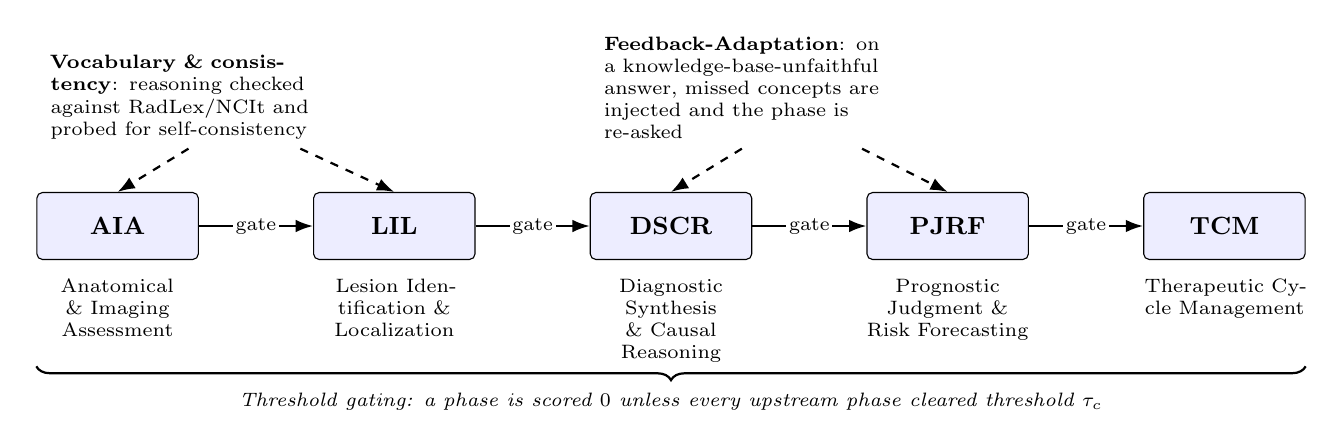
\begin{tikzpicture}[
  phase/.style={draw, rounded corners=2pt, minimum height=0.85cm, minimum width=2.05cm, align=center, font=\small\bfseries, fill=blue!7, inner sep=2pt},
  sub/.style={font=\scriptsize, align=center, text width=2.05cm},
  arr/.style={-{Latex[length=2.2mm, width=1.6mm]}, thick},
  gatelbl/.style={font=\scriptsize, fill=white, inner sep=1pt},
  axis/.style={font=\scriptsize, align=left, text width=3.5cm}
]

\node[phase] (aia) {AIA};
\node[phase, right=1.45cm of aia] (lil) {LIL};
\node[phase, right=1.45cm of lil] (dscr) {DSCR};
\node[phase, right=1.45cm of dscr] (pjrf) {PJRF};
\node[phase, right=1.45cm of pjrf] (tcm) {TCM};

\node[sub, below=0.12cm of aia] {Anatomical \& Imaging Assessment};
\node[sub, below=0.12cm of lil] {Lesion Identification \& Localization};
\node[sub, below=0.12cm of dscr] {Diagnostic Synthesis \& Causal Reasoning};
\node[sub, below=0.12cm of pjrf] {Prognostic Judgment \& Risk Forecasting};
\node[sub, below=0.12cm of tcm] {Therapeutic Cycle Management};

\draw[arr] (aia) -- (lil);
\draw[arr] (lil) -- (dscr);
\draw[arr] (dscr) -- (pjrf);
\draw[arr] (pjrf) -- (tcm);

\node[gatelbl] at ($(aia.east)!0.5!(lil.west)$) {gate};
\node[gatelbl] at ($(lil.east)!0.5!(dscr.west)$) {gate};
\node[gatelbl] at ($(dscr.east)!0.5!(pjrf.west)$) {gate};
\node[gatelbl] at ($(pjrf.east)!0.5!(tcm.west)$) {gate};

\draw[decorate, decoration={brace, amplitude=5pt, mirror}, thick]
  ($(aia.south west)+(0,-1.35cm)$) -- ($(tcm.south east)+(0,-1.35cm)$)
  node[midway, below=6pt, font=\scriptsize\itshape] {Threshold gating: a phase is scored $0$ unless every upstream phase cleared threshold $\tau_c$};

\node[axis, above=0.55cm of aia, xshift=0.9cm] (faith)
  {\textbf{Vocabulary \& consistency}: reasoning checked against RadLex/NCIt and probed for self-consistency};
\draw[arr, dashed] (faith.south) -- (aia.north);
\draw[arr, dashed] (faith) -- (lil.north);

\node[axis, above=0.55cm of dscr, xshift=0.9cm] (adapt)
  {\textbf{Feedback-Adaptation}: on a knowledge-base-unfaithful answer, missed concepts are injected and the phase is re-asked};
\draw[arr, dashed] (adapt.south) -- (dscr.north);
\draw[arr, dashed] (adapt) -- (pjrf.north);

\end{tikzpicture}%
}
\caption{The KAB framework: a brain-MRI case is evaluated as a five-phase sequential chain (bottom), with three metrics attached to it (top and below): vocabulary and consistency (ontology term validity + answer-reasoning self-consistency), feedback-adaptation (a targeted re-query on failure), and threshold gating (a phase counts only if its upstream phases cleared a score threshold).}
\label{fig:overview}
\end{figure*}



KAB evaluates a model per case, a case being one patient's progression through the five phases. For each question the model receives the image(s), question, options, and a summary of its own earlier answers in the case (the \emph{chain context}), and returns an answer, a description of what it observed in the image (\texttt{visual\_grounding}), and reasoning. KAB computes three families of measures on top of this interaction.

\subsection{Vocabulary and Consistency Metrics}
\label{sec:faithfulness}

\emph{Answer recoverability}: a second call sees only the model's reasoning text and asks which answer it supports; a match means the reasoning is textually sufficient for the answer. This establishes self-consistency, not that the reasoning caused the answer. \emph{Ontology term coverage}: the fraction of the response's knowledge-base terms that belong to the phase-appropriate base (RadLex for AIA and LIL, the NCI Thesaurus for DSCR, PJRF, and TCM); it measures term validity, not correctness. We also compute answer-term overlap and upstream-term repetition (Appendix~\ref{sec:app-metrics}). We call these vocabulary and consistency measures because none tests causal faithfulness.

\subsection{Feedback-Based Adaptation}
\label{sec:adaptation}

When ontology coverage falls below $\tau_g=0.3$ and missed concepts exist (phase-KB terms in the correct answer but absent from the response), we re-ask with the model's prior answer and a correction block listing the missed concepts, and report the fraction corrected. This measures performance under a targeted, answer-derived hint. Because the hint supplies new information, it does not separate a knowledge gap from an activation failure; that would need generic-retry and irrelevant-hint controls, which we have not run.

\subsection{Threshold Gating}
\label{sec:gating}

A phase's score is set to $0$ (\texttt{gated\_out}) unless every phase it is assumed to depend on scored at least $\tau_c=0.5$: LIL requires AIA; DSCR requires AIA and LIL; PJRF the first three; TCM all four. The rule is binary, so it is hard gating. It is an imposed scoring convention, not a demonstrated dependency: a model can misidentify a sequence yet localize a lesion, or answer every phase through independent shortcuts, and our DSCR answer keys do not depend on the LIL baseline (Appendix~\ref{sec:app-v3-construction}). We test the dependency by manipulating upstream context (Appendix~\ref{sec:gating-causality}). In the implementation a blocked phase is not queried, but a queried phase's inputs do not depend on gating, so a gated run equals a non-gated run with blocked scores set to zero; all results here use non-gated runs. A high chain completion rate (every phase ran and cleared its gate) means above-threshold scores at every phase, not necessarily coherent reasoning.


\section{Metric Definitions}
\label{sec:app-metrics}

\subsection{Vocabulary and Consistency Metrics}

\paragraph{Answer recoverability.} After a model answers, we issue a second call, the recoverability probe, containing \emph{only} the model's own reasoning text (no image, no question, no answer options) and ask which answer that reasoning supports. If the probe's predicted answer matches the model's original answer, the response is \emph{recoverable}: the stated reasoning is sufficient, on its own, for a downstream reader (here, the probe model) to reconstruct the same conclusion. A mismatch means the model's justification is disconnected from the answer it actually gave. This establishes textual self-consistency between an answer and its stated reasoning; it does not establish that the reasoning caused the answer, since a response can restate its own conclusion in different words without that restatement having driven the decision. We separately flag \emph{correct-but-unrecoverable} responses, a right answer paired with reasoning that does not support it, as the most clinically dangerous category, since such a response offers no evidence it will generalize to a case that differs even slightly from the one it was scored on.

\paragraph{Ontology term coverage.} This is KAB's central grounding-adjacent metric; despite the name, it measures term \emph{validity}, not correctness (see Section~\ref{sec:limitations}). Every diagnostic phase has an authoritative source of real clinical vocabulary: RadLex \citep{rsna_radlex} for radiology anatomy, imaging modalities, and lesion descriptors (routed to the AIA and LIL phases), and the NCI Thesaurus (NCIt; \citealp{sioutos2007nci}) for tumor classification, WHO grading, molecular markers, staging, and treatment (routed to DSCR, PJRF, and TCM). NCIt was chosen over UMLS because OmniBrainBench and LUMIERE are both predominantly glioma/glioblastoma datasets, for which NCIt has the deepest freely-available coverage, and because it requires no account or API key, removing a reproducibility barrier. We concatenate a model's \texttt{visual\_grounding} and \texttt{reasoning} fields, tokenize the text (preserving hyphenated compounds such as \emph{ring-enhancing} as single tokens), and run a greedy longest-match scan against the union of both knowledge bases, trying 4-grams down to 1-grams with no reuse of consumed token positions. This yields \texttt{extracted\_concepts}: every KB term the model used regardless of phase. We then take \texttt{matched\_concepts} as the subset of \texttt{extracted\_concepts} present in the phase-appropriate KB, and compute
\begin{equation}
  \label{eq:kb-align}
  \text{OntCoverage} = \frac{|\text{matched\_concepts}|}{|\text{extracted\_concepts}|}.
\end{equation}
A low score indicates the model is not using vocabulary appropriate to the current diagnostic phase, for example still describing anatomy at the diagnosis phase rather than committing to tumor-classification language; unrecognized assertions are excluded from the denominator entirely, so this score says nothing about whether the model's \emph{unrecognized} content is accurate, only about the recognized fraction.

\paragraph{Answer-term overlap.} Ontology term coverage measures whether a model used \emph{real} clinical terms; answer-term overlap measures whether it used ones that also appear in \emph{this case's correct answer text} — a proxy for on-target vocabulary, not for whether the surrounding explanation is a genuinely correct account of the case. Of the matched phase-KB concepts, we compute the fraction that also appear in the correct answer text:
\begin{equation}
  \label{eq:concept-precision}
  \text{AnswerTermOverlap} = \frac{|\text{on-target matches}|}{|\text{matched\_concepts}|}.
\end{equation}
A model can score high on ontology term coverage while scoring low on answer-term overlap: using plausible-sounding real clinical language that is nonetheless wrong for the case at hand. The converse is also possible: repeating answer-option wording verbatim scores high on this metric without necessarily reflecting reasoning.

\paragraph{Upstream-term repetition.} For each phase after AIA, we check what fraction of the key terms from the correct answers of \emph{upstream} phases are referenced in the current phase's reasoning text. This measures textual repetition of upstream terms, not demonstrated reasoning dependency: a model that identified a lesion in the right temporal lobe during LIL but never references that location during DSCR is \emph{at least} answering each phase in isolation rather than visibly carrying context forward, but the converse does not hold, repeating an upstream term does not by itself show the current answer was reasoned \emph{from} it, nor does omitting one show independent reasoning.

\subsection{Feedback-Based Adaptation}

The metrics above establish whether a model's stated reasoning uses valid, on-target clinical vocabulary and is self-consistent with its answer, not whether the model reasoned correctly; the adaptation loop asks a different question: whether a model with low ontology term coverage can be corrected when the missing vocabulary is handed to it directly. The loop triggers when a response has low ontology term coverage (OntCoverage below a threshold $\tau_g$, default $0.3$) \emph{and} has a non-empty set of missed concepts, defined as phase-KB terms present in the correct answer but absent from the model's output. When triggered, we re-issue the original prompt augmented with the model's prior answer and reasoning and an explicit \texttt{CLINICAL KNOWLEDGE CORRECTION} block listing the missed concepts, and ask the model to re-examine the image in light of this correction. We record whether the model changed its answer (\texttt{adaptation\_changed}) and whether the revised answer is correct (\texttt{adaptation\_correct}), and report the \emph{adaptation rate}: the fraction of triggered questions that the model corrects to the right answer. We describe this as performance under a targeted, answer-derived hint; correcting after such a hint does not by itself establish that the model already possessed the relevant knowledge and merely failed to activate it, since the hint also supplies new information. Distinguishing a genuine \emph{knowledge gap} from an \emph{activation failure} would require comparing this targeted-hint condition against a generic-retry control (re-asking without new information) and an irrelevant-hint control (a correction block naming concepts not relevant to the case); we have not yet run these controls, so we report the targeted-hint adaptation rate alone rather than the knowledge-gap/activation-failure distinction.



\section{OmniBrainBench Compatibility Details}
\label{sec:app-compat}

The KAB framework as described in Section~\ref{sec:kab} presupposes that a case's five phases represent one patient's actual clinical trajectory: a model that fails AIA for a given patient should be gated out of that same patient's DSCR question, not an unrelated patient's. We investigated whether OmniBrainBench \citep{peng2026omnibrainbench} supports this premise, by checking whether any image is shared across questions tagged with different clinical phases within a grouped case. Shared images are the evidence of continuity that the released data let us verify directly; they are not the only conceivable evidence, and the absence of shared images is not proof that no two questions concern the same patient.

OmniBrainBench ships 9,527 total QA pairs; we use its 6,823-question \emph{closed-ended} (multiple-choice) subset, since KAB's gating and scoring require answer options, and exclude the remaining 2,704 open-ended pairs. Of these 6,823 questions, drawn from 15 source sub-corpora (including PubMedVision, BraTS2021, RSNA, ISLES2022, and VQA\_RAD, among others), we found only \textbf{2} verifiable cross-phase patient links, i.e.\ patients whose images appear in questions from two different phases, both from VQA\_RAD, each contributing one AIA question and one LIL question (4 questions total across the 2 pairs). We repeated the analysis with a second, independent method (extracting real per-patient case identifiers by stripping known modality/view/slice suffixes from filenames on a per-corpus basis) and obtained the same result: 2 verifiable multi-phase same-patient links in the entire dataset (4 questions), none spanning three or more phases, none spanning all five. Because the release provides no complete patient identifier, we cannot rule out further true links that neither method detects; the counts are lower bounds on verifiable links, not a census of patients. The root cause is structural: each of the 15 source sub-corpora was constructed for one specific clinical task (e.g., BraTS for tumor characterization, RSNA for hemorrhage classification, ISLES for stroke), so a given real patient within a sub-corpus is essentially only ever asked one phase-type of question. \texttt{source\_file} is a field present in OmniBrainBench's own released data, denoting each question's origin annotation batch; using it to represent same-patient identity for a multi-phase causal chain is our own KAB-side interpretation, not a claim OmniBrainBench itself makes about that field. Under that interpretation, \texttt{source\_file} in practice groups together an entire origin sub-corpus, standing in for a single patient; what this grouping evaluates as a chain is stitched from \emph{different real patients'} questions, not one patient's actual diagnostic journey. A model gated out of a later phase after failing an earlier one under this grouping demonstrates nothing about reasoning across any single patient's chain. We frame this as an incompatibility between the released benchmark and our proposed sequential evaluation, not as a defect in a promise OmniBrainBench made: we are not aware of an explicit claim by its authors that the released closed-ended questions form patient-linked longitudinal chains. The benchmark paper's supplement does describe a separate patient-level extension, OmniBrainBench-Extended, built on the ADNI Alzheimer's cohort with subject IDs across the five phases; because ADNI is access-restricted, only annotations and metadata are to be released. As of September 2026 the authors' public repository contains only label-generation scripts for it, covering structure and modality identification, cognitive-status diagnosis (cognitively unimpaired, mild cognitive impairment, dementia), white-matter-hyperintensity localization, and a future-decline risk label; its ``treatment-related'' task generates risk categories, and we found no therapy-selection questions. The UK Biobank part is marked unfinished and no question data are provided. We did not evaluate it, and it is not a brain-tumor cohort.

We searched for a replacement or supplementary dataset with genuine same-patient, multi-phase continuity and a ready-made question layer (Section~\ref{sec:related-work}); none exists. This motivates the construction described next.


\section{Evidence-Audit, Option-Only, and TCM-Lookup Details}
\label{sec:app-audit}

\paragraph{Evidence audit.} Necessity and use are different claims: an image could be unnecessary on average while still being consulted, so we separately audit the content of a model's stated evidence against the same structured per-patient facts used to draft the items (Section~\ref{sec:lumiere}). For each checkable claim in a response's \texttt{visual\_grounding} and \texttt{reasoning} fields (hemisphere/region statements and any measurement with units), we record two separate properties. \emph{Availability}: whether the claim's content already appears in the stem, answer options, or upstream chain context the model was shown. \emph{Record status}: whether the claim is \emph{supported} by the ground-truth facts (a measurement within 2\% of a fact value, or a hemisphere present in the segmentation), \emph{contradicted} (a hemisphere opposite to the segmentation, under the assumption that image left corresponds to patient right), \emph{unmatched} (a measurement matching no fact value; pattern matching cannot show that such a value is wrong, since it may be a derived quantity), or \emph{unverifiable} (a hemisphere claim with no segmentation to compare). Keeping the dimensions separate matters: an earlier single-label scheme reported any claim already present in shown text as ``copied'', which hid the case in which a wrong claim is repeated from an earlier turn, and it read ``not copied'' as independent support. Responses with no checkable claim are reported separately, and claim-level denominators are stated. We treat hemisphere mismatches with care because the rendered slices follow radiological display convention without stating so in the prompt for the initial item set (fixed for the leak-controlled set, Section~\ref{sec:lumiere}): a hemisphere claim that is wrong under one convention and right under the other reflects a display ambiguity, not a perceptual error. RANO-criteria thresholds quoted verbatim from clinical guidelines (e.g., ``$\geq$25\% increase'') are excluded, since they restate a rule rather than assert a patient-specific fact. The audit is deterministic pattern matching, not an LLM judge: numeric claims are compared by value against the facts and the shown-text pool, and hemisphere claims against the segmentation's own left/right extent. This makes it reproducible from a response's text, but it does not interpret paraphrase or synonymy (Section~\ref{sec:limitations}).

\paragraph{Option-only baselines.} Guessers that use only the options and stem, computed on the \texttt{v3} items exactly as shown (options shuffled; $n=52$ per phase), are informative about answer-key artifacts. Always choosing the longest option scores 37\% on AIA, 25\% on LIL, 67\% on DSCR (matching the majority class, since progressive disease is typically the longest option), 19\% on PJRF, and 6\% on TCM. The most common correct letter, fitted on the same items and therefore optimistic, scores 31--37\% on every phase. Choosing the option with the most words shared with the stem scores 0--33\%. Except for the AIA and DSCR entries, which reflect a constant correct string and a class imbalance, these sit near the four-option chance level (a guesser fitted on the same items reaches up to 37\%). DSCR's longest-option score equals the majority class (\dscrMajorityPct{}\%), which no model exceeds. AIA's correct answer is the same string in every item, so a baseline that recognizes that text rather than a letter would score 100\%. The LLM options-only baseline and the no-chain-context comparator are in Table~\ref{tab:optonly}.

\begin{table}[t]
\centering
\setlength{\tabcolsep}{2pt}
\scriptsize
\begin{tabular}{llcccc}
\toprule
Model & Phase & Opt.-only & No chain & Own-img & Unpars. \\
\midrule
MedGemma-4B & AIA & 40.4$^\dagger$ & 51.9 & 51.9 & 19 \\
 & LIL & 28.8 & 42.3 & 40.4 & 0 \\
 & DSCR & 0.0$^\dagger$ & 19.2 & 15.4 & 52 \\
 & PJRF & 13.5$^\dagger$ & 34.6 & 36.5 & 18 \\
 & TCM & 15.4$^\dagger$ & 25.0 & 26.9 & 21 \\
Gemma-3-12B & AIA & 38.5 & 90.4 & 90.4 & 0 \\
 & LIL & 32.7 & 23.1 & 23.1 & 0 \\
 & DSCR & 40.4 & 65.4 & 55.8 & 0 \\
 & PJRF & 23.1 & 30.8 & 32.7 & 0 \\
 & TCM & 11.5 & 19.2 & 38.5 & 0 \\
Gemma-3-27B & AIA & 61.5 & 86.5 & 86.5 & 0 \\
 & LIL & 36.5 & 25.0 & 26.9 & 0 \\
 & DSCR & 44.2 & 71.2 & 65.4 & 0 \\
 & PJRF & 25.0 & 34.6 & 28.8 & 0 \\
 & TCM & 11.5 & 32.7 & 59.6 & 0 \\
Llama-4-Scout & AIA & 44.2 & 94.2 & 94.2 & 0 \\
 & LIL & 36.5 & 28.8 & 25.0 & 0 \\
 & DSCR & 19.2 & 63.5 & 57.7 & 7 \\
 & PJRF & 21.2 & 34.6 & 30.8 & 0 \\
 & TCM & 19.2 & 32.7 & 36.5 & 0 \\
\bottomrule
\end{tabular}

\caption{Accuracy (\%, $n=52$ per cell) with the options alone; with image and stem but no chain context (the ``absent'' condition of the gating-causality run, and the ordinary own-image run for AIA, which has no upstream phase); and in the ordinary own-image run, which carries the model's own earlier answers as chain context. Chance is 25\%; the majority answer text is 100\% for AIA, \dscrMajorityPct{}\% for DSCR, and 1.9\% for LIL, PJRF, and TCM. Opt.-only is options only; Own-img is the ordinary own-image run; Unpars. is the number of unparseable options-only responses; unparseable responses score incorrect. $^\dagger$ More than 20\% unparseable: a lower bound, and its paired comparison with the own-image run is suppressed as an artifact. Own-image minus options-only mixes image, stem, and the model's own upstream answers, so it is not an image effect.}
\label{tab:optonly}
\end{table}

\paragraph{TCM label lookup.} A fixed keyword rule assigns each TCM option an action class from its first ten words (escalate: second-line or salvage therapy, re-resection, radiosurgery, re-irradiation, trial; stop: discontinue, suspend, best supportive care; continue: continue, maintain; otherwise other; rules in \texttt{tools/lumiere\_tcm\_lookup.py}). The DSCR key predicts the TCM key\textquoteright s class (progressive disease $\to$ escalate, other ratings $\to$ continue) in \tcmAgree{} of \tcmN{} patients (\tcmPdEsc{} of \tcmPdN{} and \tcmNonCont{} of \tcmNonN{}), but the key\textquoteright s class is unique among the four options in only \tcmClassUnique{} of \tcmN{}, so the class alone fixes the letter in a minority of items. (An earlier version of this tool compared answer strings and treated the two keys spelled ``Progressive disease (PD)'' as non-progressive, which gave 50 of 52; labels are now compared after canonicalization.) Among the \tcmPdN{} patients whose DSCR key is progressive disease, the number of TCM answers in the escalate class under correct, forced-wrong, and absent DSCR context is \tcmFollowCorrectGemmaTwelve{}, \tcmFollowIncorrectGemmaTwelve{} and \tcmFollowAbsentGemmaTwelve{} for Gemma-3-12B; \tcmFollowCorrectGemmaTwentySeven{}, \tcmFollowIncorrectGemmaTwentySeven{} and \tcmFollowAbsentGemmaTwentySeven{} for Gemma-3-27B; \tcmFollowCorrectScout{}, \tcmFollowIncorrectScout{} and \tcmFollowAbsentScout{} for Llama-4-Scout; and \tcmFollowCorrectMedGemma{}, \tcmFollowIncorrectMedGemma{} and \tcmFollowAbsentMedGemma{} for MedGemma-4B, which does not follow the injected label. TCM accuracy split by whether the model\textquoteright s own DSCR answer was correct gives Fisher exact $p=.0013$ (Gemma-3-12B), $.0010$ (Gemma-3-27B), $3\times10^{-5}$ (Llama-4-Scout), and $.19$ (MedGemma-4B); these splits are descriptive and confounded by patient difficulty.


\section{A Worked Patient Example}
\label{sec:worked-example}

To make the abstract description of items, chain context, and evidence auditing in Appendices~\ref{sec:kab} and~\ref{sec:app-v3} concrete, this appendix walks through one complete case end to end: Patient-002's leak-controlled (\texttt{v3}) five-phase chain, as answered by Gemma-3-27B (the best-performing open-weight model), together with the evidence fact-check's actual (audit-tool-generated, not hand-picked) classification of the model's stated reasoning at each phase.

\paragraph{The patient.} Patient-002 is a 71-year-old female with glioblastoma (MGMT unmethylated, IDH status unavailable) who underwent complete resection of the enhancing tumor followed by Stupp-protocol chemoradiation. The post-operative rebaselined LIL comparison is week-040-2 (baseline) versus week-047 (follow-up): total lesion volume increases from 27,937mm$^3$ to 57,570mm$^3$ (+106\%), with the enhancing core and necrotic components moving from the Superior Parietal Lobule at baseline to the Left Cerebral White Matter at follow-up. The week-047 RANO rating is progressive disease. Recorded overall survival from surgery is 48 weeks.

\paragraph{AIA.} \emph{Question:} which imaging modalities were available. \emph{Correct/model answer:} T1, contrast-enhanced T1, T2, and FLAIR (correct). The model's stated \texttt{visual\_grounding} for this item, unprompted, also volunteers a lesion location: \textit{``a mass lesion in the right temporal lobe.''} No part of the AIA question or options mentions location, so this claim is neither asked for nor copied from anything shown to the model. Checked against the same structured facts used to draft the item, it is wrong on two counts: the true baseline location is the Superior Parietal Lobule/Left Cerebral White Matter (not temporal), and the true laterality is left, not right. Running the evidence fact-check's hemisphere check on this claim in isolation (Appendix~\ref{sec:grounding-test}) labels it \emph{laterality\_flip}: a real, audit-caught contradiction, reported under that label rather than as ordinary fabrication per the paper's own convention (Appendix~\ref{sec:grounding-test}), since a display-orientation ambiguity cannot be ruled out for this claim in the same way it can for later ones below.

\paragraph{LIL.} \emph{Question:} how did the lesion's location and volume change between baseline and follow-up. \emph{Correct/model answer:} shifted predominantly to the Left Cerebral White Matter, +106\% (correct). The model's reasoning restates the same fabricated baseline location from AIA (\textit{``the initial lesion is located in the right temporal lobe''}), now unchanged across a full phase boundary, and concludes with the correct answer's own location and percentage. Run through the fact-check, every checkable claim in this response, the repeated ``right temporal lobe'' and the ``106\%'' figure alike, is labeled \emph{copied} under the earlier single-label scheme: not because the audit missed the AIA-level contradiction, but because by LIL, both claims are present in the model's own prior-turn output or the shown answer options, which is why that label cannot distinguish a genuinely re-verified observation from one simply carried forward. Under the two-dimension scoring of Appendix~\ref{sec:grounding-test} the same response contains 3 claims that are available in shown text and match the record and 2 (the repeated ``right temporal lobe'') that are available in shown text but contradict it, so the carried-forward error remains visible.

\paragraph{DSCR.} \emph{Question:} RANO response category at week-047. \emph{Correct/model answer:} progressive disease (correct). The model's evidence again repeats the ``right temporal lobe'' framing and the radiology-report measurement it was shown, and the fact-check again labels every claim \emph{copied}. The final answer is correct, and consistent with the (still-wrong) location claim the model has now repeated across three consecutive phases without correction.

\paragraph{PJRF.} \emph{Question:} expected overall survival from surgery. \emph{Correct answer:} approximately 12 months (48-52 weeks) — age over 70 as the dominant adverse factor despite complete resection. \emph{Model answer:} approximately 9 months (36-40 weeks) — the option attributing a \emph{particularly} poor prognosis to the same unmethylated-MGMT/age-over-70 combination. This is the one incorrect answer in the chain, but it illustrates a limit of the answer key rather than only a model error: both options describe the same adverse risk factors in the same direction, the key is the bucket consistent with the \emph{realized} 48-week survival, and a nine-month forecast is a plausible prognosis for a 71-year-old with unmethylated MGMT that the key marks wrong. The example also shows why the information cutoff matters: the follow-up imaging is at week 47 and survival is measured from surgery, so the outcome falls one week after the last image.

\paragraph{TCM.} \emph{Question:} appropriate management at this time. \emph{Correct/model answer:} initiate second-line therapy given evidence of true progression (correct).

\paragraph{Reading this case.} Taken as a whole, this single chain illustrates the gap the \texttt{v3} results report in aggregate: 4 of 5 final answers are correct, but the evidentiary trail behind the LIL and DSCR answers rests on a spatial claim introduced at AIA that the fact-check itself flags as contradicting the ground truth, not on independently re-derived observation at each phase. We did not select this patient for this property after the fact; it is Patient-002, the first case in the evaluation order, and its fact-check labels above are exactly what \texttt{tools/audit\_reasoning\_facts.py} outputs when run on it, not a paraphrase.


\section{Item-Set Development History}
\label{sec:dev-history}

This appendix records the construction problems found and fixed while building the LUMIERE item set, in the order they were found. Appendix~\ref{sec:app-v3-construction} describes only the final procedure; Figure~\ref{fig:lumiere-pipeline} summarizes it.

\begin{figure*}[t]
\centering
\resizebox{\textwidth}{!}{%
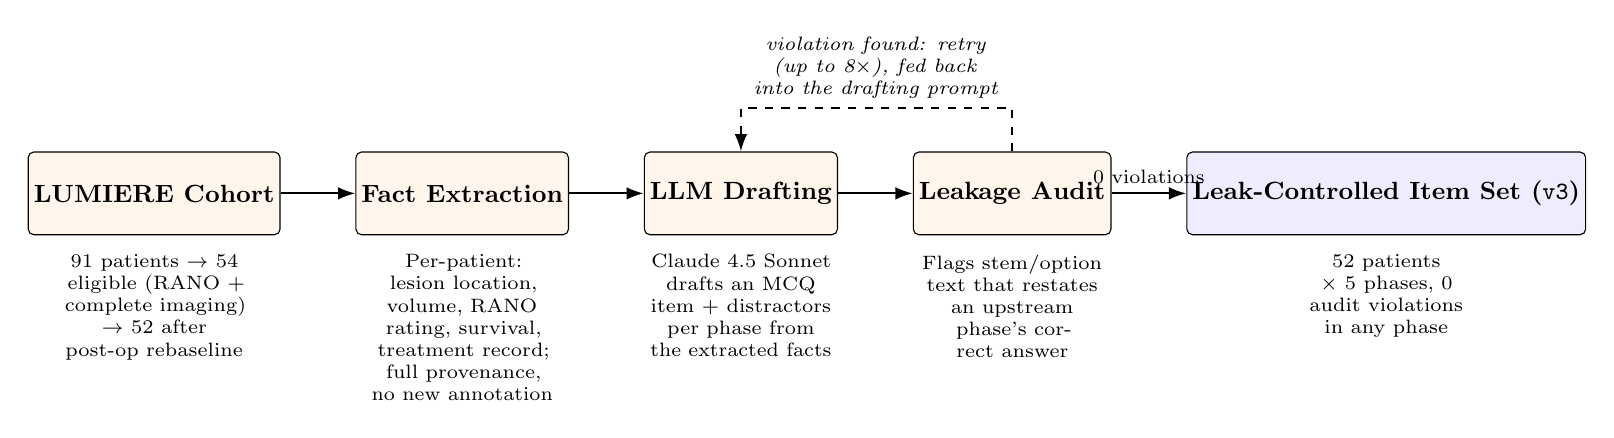
\begin{tikzpicture}[
  stage/.style={draw, rounded corners=2pt, minimum height=1.05cm, minimum width=2.3cm, align=center, font=\small\bfseries, fill=orange!8, inner sep=2pt},
  final/.style={draw, rounded corners=2pt, minimum height=1.05cm, minimum width=2.3cm, align=center, font=\small\bfseries, fill=blue!7, inner sep=2pt},
  sub/.style={font=\scriptsize, align=center, text width=2.3cm},
  arr/.style={-{Latex[length=2.2mm, width=1.6mm]}, thick}
]

\node[stage] (cohort) {LUMIERE Cohort};
\node[stage, right=0.95cm of cohort] (facts) {Fact Extraction};
\node[stage, right=0.95cm of facts] (draft) {LLM Drafting};
\node[stage, right=0.95cm of draft] (audit) {Leakage Audit};
\node[final, right=0.95cm of audit] (out) {Leak-Controlled Item Set (\texttt{v3})};

\node[sub, below=0.12cm of cohort] {91 patients $\to$ 54 eligible (RANO + complete imaging) $\to$ 52 after post-op rebaseline};
\node[sub, below=0.12cm of facts] {Per-patient: lesion location, volume, RANO rating, survival, treatment record; full provenance, no new annotation};
\node[sub, below=0.12cm of draft] {Claude 4.5 Sonnet drafts an MCQ item + distractors per phase from the extracted facts};
\node[sub, below=0.12cm of audit] {Flags stem/option text that restates an upstream phase's correct answer};
\node[sub, below=0.12cm of out] {52 patients $\times$ 5 phases, 0 audit violations in any phase};

\draw[arr] (cohort) -- (facts);
\draw[arr] (facts) -- (draft);
\draw[arr] (draft) -- (audit);
\draw[arr] (audit) -- (out) node[midway, above, font=\scriptsize] {0 violations};

\draw[arr, dashed] (audit.north) -- ++(0,0.55cm) -| (draft.north);
\node[font=\scriptsize\itshape, align=center, text width=3.6cm, above]
  at ($(audit.north)!0.5!(draft.north)+(0,0.55cm)$)
  {violation found: retry (up to 8$\times$), fed back into the drafting prompt};

\end{tikzpicture}%
}
\caption{Construction pipeline for the leak-controlled (\texttt{v3}) LUMIERE item set. Structured per-patient facts are extracted from LUMIERE, an LLM drafts multiple-choice items from those facts, and an automatic auditor flags any item that restates an upstream phase's correct answer, feeding violations back into the drafting prompt for up to eight retries.}
\label{fig:lumiere-pipeline}
\end{figure*}


\paragraph{Timepoint sampling.} We initially selected each patient's most recent RANO-rated timepoint, but found this made nearly every DSCR answer \emph{progressive disease}, since glioblastoma patients overwhelmingly trend toward progression by their final scan, a sampling choice that would have made the DSCR phase trivially guessable regardless of a model's actual reasoning. We instead sample a random eligible response-rated timepoint per patient (fixed seed), which yields a substantially more balanced label distribution across the 54-patient cohort: 37 progressive disease, 9 stable disease, 4 partial response, and 4 complete response. We additionally found and fixed a related bug in which a randomly sampled RANO-rated timepoint could lack matching complete imaging, silently falling back to imaging from a \emph{different} date than the one the RANO rating and DSCR facts describe; we now constrain sampling to timepoints with both a rating and complete imaging, and verified zero such mismatches across the full extracted cohort.


\paragraph{Stem-leakage audit and a leak-controlled item set.} Manual inspection of the drafted items surfaced a systematic construction flaw: the drafter wrote each phase's question stem as a self-contained clinical vignette, which led it to restate findings established in earlier phases of the same chain. We built an automatic auditor that flags, per phase, any stem or option text containing content it should not have access to: a numeric percent volume change, a raw volume or region name, a change-direction word, a RANO label, or a stated survival duration, checked both against the phase's own correct answer (\emph{self-leakage}) and against the correct answers of upstream phases in the same chain (\emph{upstream leakage}). Applying this auditor to the initial item set (\texttt{v2}) found leakage in a majority of DSCR, PJRF, and TCM items and a smaller fraction of LIL items; a lexical baseline that guesses the option with the highest word overlap with the stem performs at or below chance on the same items, confirming the leak is semantic (e.g., a stated percent volume increase implying \emph{progressive disease}) rather than a copy-paste artifact a naive overlap check would already catch.

We traced the cause to the drafting prompt itself, which supplied each phase's drafting call with the correct answers of upstream phases (necessary for constructing a coherent chain) without instructing the model not to restate them, and, for DSCR specifically, explicitly asked the model to let the reader \emph{infer} the response label from volume-change facts it had just been shown. We built a revised, leak-controlled item set (\texttt{v3}) that keeps the same upstream-truth context available to the drafter but forbids restating it in the visible stem or options, re-drafting automatically (up to eight attempts) whenever the auditor flags a violation and feeding the specific violated rule back into the retry prompt. The DSCR stem, which the auditor showed was hardest to keep leak-free under free-form drafting, is instead built from a fixed template populated from structured extent-of-resection, re-resection and radiotherapy-timing fields and, after the answerability check below, the rater\textquoteright s recorded findings, with no correct-answer information available to leak. The leak-controlled item set clears the auditor with zero violations across every phase. This establishes compliance with that auditor, whose rules the drafting loop was itself optimized against, not the absence of leakage.


\paragraph{Stem-leakage rates on \texttt{v2}.} The initial item set (\texttt{v2}) failed the auditor at rates too high to treat its accuracy numbers as informative about image use: 0\% of AIA items leaked, but 13\% (7/54) of LIL items self-leaked, 98\% of DSCR items restated an upstream phase's exact percent volume change, 85\% of PJRF items either stated the patient's actual survival duration directly (31\%) or named the upstream RANO label (72\%), and 98\% of TCM items restated LIL's volume-change percentage or RANO label. The leak-controlled item set (\texttt{v3}), built with the same auditor folded into the drafting retry loop (Appendix~\ref{sec:app-v3-construction}), cleared every phase with zero violations, which shows compliance with that auditor (whose rules the drafting loop was optimized against), not that no leakage remains.

\paragraph{Post-operative rebaselining.} Building the leak-controlled item set surfaced a second issue upstream of leakage: the LIL phase's volume-change baseline was, for 42 of 54 patients, a pre-operative scan, so the measured volume change mostly captured the surgical resection rather than the treatment response that the RANO rating (DSCR) is actually judged against. We recompute the LIL baseline as each patient's latest imaged post-operative scan prior to the follow-up (advancing past any re-resection that occurs before the follow-up date), changing the baseline for 44 of 54 patients and shifting the cohort's volume-change direction from a resection-dominated skew to a more balanced 20 patients increasing versus 32 decreasing. Two patients (Patient-049, Patient-068) lack a post-operative scan with matching segmentation and are excluded from the leak-controlled item set rather than mixed in on a pre-operative baseline, leaving 52 patients. Downstream DSCR, PJRF, and TCM facts and answer keys, which do not depend on the LIL baseline, are unchanged by this step (the two excluded patients were both progressive disease, taking the DSCR keys from \dscrFiftyPD{} to \dscrVthreePD{} progressive-disease items); this also shows that the answer keys of later phases are not functions of earlier phases' keys.


\paragraph{Difficulty of \texttt{v3} relative to \texttt{v2}.} \texttt{v3} items are substantially harder than \texttt{v2} for every model (image-present overall accuracy is 9--18 percentage points lower, e.g., Llama-4-Scout 66.7\%$\to$48.8\%, MedGemma-4B 45.2\%$\to$34.2\%; the two item sets cover 54 and 52 patients, so this is not a strictly paired comparison), consistent with the stem-leakage fix removing an exploitable shortcut rather than removing task difficulty. This drop is a validity correction to the earlier item set, not itself evidence about image use; we report it only to establish that the narrow with/without-image gap on \texttt{v3} is not an artifact of \texttt{v3} being an easier, less discriminating test.



\paragraph{Answerability check of DSCR.} A rough comparison of the expert RANO ratings with the baseline-to-follow-up total volume change the model sees found that only about 18 of 52 ratings agreed, and 23 of 35 progressive-disease ratings came with shrinking total volume, because the rating rests on evidence outside the rendered contrast-enhanced slice (T2/FLAIR progression, new or non-measurable lesions, comparison with the nadir). The stem of the \texttt{v3} DSCR item therefore quotes the rater\textquoteright s recorded findings (for example ``Target lesion(s): 28 mm x 44 mm after re-resection''), which makes DSCR partly answerable from text. The enhancement-based audit of Section~\ref{sec:audit} replaces this rough check.


\end{document}
